% !TeX program = xelatex

\documentclass{beamer}

\usepackage[utf8]{inputenc}
\usepackage{graphicx}
\usepackage{listings}

\lstset{
  frame=single,
  basicstyle=\footnotesize\ttfamily,
  captionpos=b,
  tabsize=2,
}
\beamertemplatenavigationsymbolsempty
\setbeamertemplate{footline}{%
\insertframenumber{}/\inserttotalframenumber}


%Information to be included in the title page:
\title{A formal analysis of IKEv2's post-quantum extension}
\usecolortheme{dove}
\author{Stefan-Lukas Gazdag, Sophia Grundner-Culemann,\\
    Tobias Guggemos, \underline{Tobias Heider},\\
    Daniel Loebenberger}
\institute{ACSAC2021}
\date{12/08/21}

\setbeamertemplate{itemize items}[circle]
\setbeamertemplate{itemize subitem}[default] \begin{document}

\begin{frame}[noframenumbering, plain]
	\titlepage
\end{frame}

\begin{frame}
\frametitle{The IKEv2 Protocol}
\includegraphics[width=\textwidth]{ike-state-machine.pdf}
\end{frame}

\begin{frame}
\frametitle{Post-Quantum IKEv2}
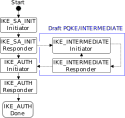
\includegraphics[width=\textwidth]{statemachine.pdf}
\end{frame}

\begin{frame}
\frametitle{The Tamarin Prover}
\end{frame}

\begin{frame}
\frametitle{IKEv2 Security Model}
\begin{itemize}
	\item Dolev-Yao-attacker
\end{itemize}
\pause
\bigskip
$\underline{\text{Security properties:}}$              
\pause
\begin{itemize}	
	\item Consistency
	\pause
	\item Key secrecy
	\pause
	\item Identity Protection
	\pause
	\item Agreement: \smallskip
	\pause
	\begin{itemize}
		\item Aliveness \textit{of Initiator and of Responder} 
		\pause        
		\item Weak Agreement \textit{of I. and of R.}
		\pause
		\item Agreement\textit{ of I. and of R.}		
	\end{itemize}
	
\end{itemize}
\end{frame}

\begin{frame}
\frametitle{Modeling IKEv2}
\end{frame}

\begin{frame}
	\frametitle{Modeling PQ-IKEv2}
\end{frame}

\begin{frame}
\frametitle{Result}
\end{frame}

\end{document}
